%%%%%%%%%%%%%%%%%%%%%%%%%%%%%%%%%%%%%%%%%
% Wenneker Assignment
% LaTeX Template
% Version 2.0 (12/1/2019)
%
% This template originates from:
% http://www.LaTeXTemplates.com
%
% Authors:
% Vel (vel@LaTeXTemplates.com)
% Frits Wenneker
%
% License:
% CC BY-NC-SA 3.0 (http://creativecommons.org/licenses/by-nc-sa/3.0/)
% 
%%%%%%%%%%%%%%%%%%%%%%%%%%%%%%%%%%%%%%%%%

%----------------------------------------------------------------------------------------
%	PACKAGES AND OTHER DOCUMENT CONFIGURATIONS
%----------------------------------------------------------------------------------------

\documentclass[11pt]{scrartcl} % Font size

%%%%%%%%%%%%%%%%%%%%%%%%%%%%%%%%%%%%%%%%%
% Wenneker Assignment
% Structure Specification File
% Version 2.0 (12/1/2019)
%
% This template originates from:
% http://www.LaTeXTemplates.com
%
% Authors:
% Vel (vel@LaTeXTemplates.com)
% Frits Wenneker
%
% License:
% CC BY-NC-SA 3.0 (http://creativecommons.org/licenses/by-nc-sa/3.0/)
% 
%%%%%%%%%%%%%%%%%%%%%%%%%%%%%%%%%%%%%%%%%

%----------------------------------------------------------------------------------------
%	PACKAGES AND OTHER DOCUMENT CONFIGURATIONS
%----------------------------------------------------------------------------------------

\usepackage{amsmath, amsfonts, amsthm} % Math packages

\usepackage{listings} % Code listings, with syntax highlighting
\usepackage[english]{babel} % English language hyphenation
\usepackage{float}
\usepackage{graphicx} % Required for inserting images
\usepackage{caption}
\graphicspath{{Figures/}{./}} % Specifies where to look for included images (trailing slash required)

\usepackage{booktabs} % Required for better horizontal rules in tables

\numberwithin{equation}{section} % Number equations within sections (i.e. 1.1, 1.2, 2.1, 2.2 instead of 1, 2, 3, 4)
\numberwithin{figure}{section} % Number figures within sections (i.e. 1.1, 1.2, 2.1, 2.2 instead of 1, 2, 3, 4)
\numberwithin{table}{section} % Number tables within sections (i.e. 1.1, 1.2, 2.1, 2.2 instead of 1, 2, 3, 4)

\setlength\parindent{0pt} % Removes all indentation from paragraphs

\usepackage{enumitem} % Required for list customisation
\setlist{noitemsep} % No spacing between list items

%----------------------------------------------------------------------------------------
%	DOCUMENT MARGINS
%----------------------------------------------------------------------------------------

\usepackage{geometry} % Required for adjusting page dimensions and margins

\geometry{
	paper=a4paper, % Paper size, change to letterpaper for US letter size
	top=2.5cm, % Top margin
	bottom=3cm, % Bottom margin
	left=3cm, % Left margin
	right=3cm, % Right margin
	headheight=0.75cm, % Header height
	footskip=1.5cm, % Space from the bottom margin to the baseline of the footer
	headsep=0.75cm, % Space from the top margin to the baseline of the header
	%showframe, % Uncomment to show how the type block is set on the page
}

%----------------------------------------------------------------------------------------
%	FONTS
%----------------------------------------------------------------------------------------

\usepackage[utf8]{inputenc} % Required for inputting international characters
\usepackage[T1]{fontenc} % Use 8-bit encoding
\usepackage{adforn}

\usepackage{fourier} % Use the Adobe Utopia font for the document

%----------------------------------------------------------------------------------------
%	SECTION TITLES
%----------------------------------------------------------------------------------------

\usepackage{sectsty} % Allows customising section commands

\sectionfont{\vspace{6pt}\centering\normalfont\scshape} % \section{} styling
\subsectionfont{\normalfont\bfseries} % \subsection{} styling
\subsubsectionfont{\normalfont\itshape} % \subsubsection{} styling
\paragraphfont{\normalfont\scshape} % \paragraph{} styling

%----------------------------------------------------------------------------------------
%	HEADERS AND FOOTERS
%----------------------------------------------------------------------------------------

\usepackage{scrlayer-scrpage} % Required for customising headers and footers

\ohead*{} % Right header
\ihead*{} % Left header
\chead*{} % Centre header

\ofoot*{} % Right footer
\ifoot*{} % Left footer
\cfoot*{\pagemark} % Centre footer
 % Include the file specifying the document structure and custom commands

%----------------------------------------------------------------------------------------
%	TITLE SECTION
%----------------------------------------------------------------------------------------

\title{	
	\normalfont\normalsize
	\textsc{Ca' Foscari University of Venice}\\ % Your university, school and/or department name(s)
	\vspace{25pt} % Whitespace
	\rule{\linewidth}{0.5pt}\\ % Thin top horizontal rule
	\vspace{20pt} % Whitespace
	{\huge A Blockchain Application - Report}\\ % The assignment title
	\vspace{12pt} % Whitespace
	\rule{\linewidth}{2pt}\\ % Thick bottom horizontal rule
	\vspace{12pt} % Whitespace
}

\author{\hspace{-0.8cm} \parbox{4cm}{\centering
  Sandro Baccega\\ 855957} \parbox{4cm}{\centering
  Diletta Olliaro\\ 855957} \parbox{4cm}{\centering
  Giacomo Zanatta\\ 855957} \parbox{4cm}{\centering Giulio Zausa\\ 855957} } % Your name



\date{\vspace{20pt}\today} % Today's date (\today) or a custom date

\begin{document}

\maketitle % Print the title



\section{Introduction}

In this report we are going to present the created blockchain application and to study its performance through the analysis of the results of different benchmarks carried on with the Tsung stress testing tool.

\subsection{Hardware}
The server runs inside a native Linux Docker Container. The underlying host is a Linux machine with the following hardware:
\begin{itemize}
\item[\adforn{43}] CPU: Intel Core i5-2520M 2.5 GHz, 2 cores and 4 threads
\item[\adforn{43}] RAM: 6 GB DDR3
\item[\adforn{43}] Disk: SanDisk 256 GB SATA SSD
\item[\adforn{43}] Network: 1 Gbps Wired Ethernet
\end{itemize}

\subsection{Software}

The host is running Ubuntu 20.04 as Operating System, while the application is deployed using Docker. 
This allows us to easily manage deployments and eventual horizontal scaling, by spawning multiple nodes in a cluster. 
Even if our application runs in a Docker container, this will not compromise the performance since we will run it on a native Linux host. 
We choosed Docker to future-proof our application, since it will make the deploy a node in the application's network easy, since it will not require to install any dependencies in the hosting system and it will not have any problem with the versions of those dependencies, saving us a lot of time in the long run.

\section{First Task}

Develop a web application based on the blockchain technology, meaning that in practice we are going to create a non-modifiable database of flying statistics. In the blockchain we must be able to:
\begin{itemize}
\item[\adforn{43}] add a new transaction
\item[\adforn{43}] retrieve a transaction based on the transaction ID
\item[\adforn{43}] retrieve all the transactions of a block
\end{itemize}

Moreover the mining operation should be invoked automatically every minute. 

Then the web application should allow the following operations:
\begin{itemize}
\item[\adforn{43}] add a new record to the chain
\item[\adforn{43}] query the status of a flight given the flight number and the date
\item[\adforn{43}] query the average delay of a flight carrier in a certain interval of time
\item[\adforn{43}] Given a pair of cities A and B, and a time interval, count the number of flights connecting city A to city B
\end{itemize}

\subsection{Implementation}

For implementing the \textit{blockchain} system we used \textbf{NodeJS} with TypeScript. NodeJS is a server runtime that runs JavaScript code. The main feature of NodeJS is its \textbf{Event Queue} \textit{(libuv)}: every IO operation is enqueued in a FCFS queue and processed by multiple threads (figure \ref{fig:eventloop}). The application logic, though, remains single-threaded. In this way the requests are processed with a FCFS policy, as we have seen also from the benchmark data. Using Javascript for this type of applications certainly is not the best choise performance wise, but it's a much simpler alternative compared to other programming languages.

\begin{figure}[h]
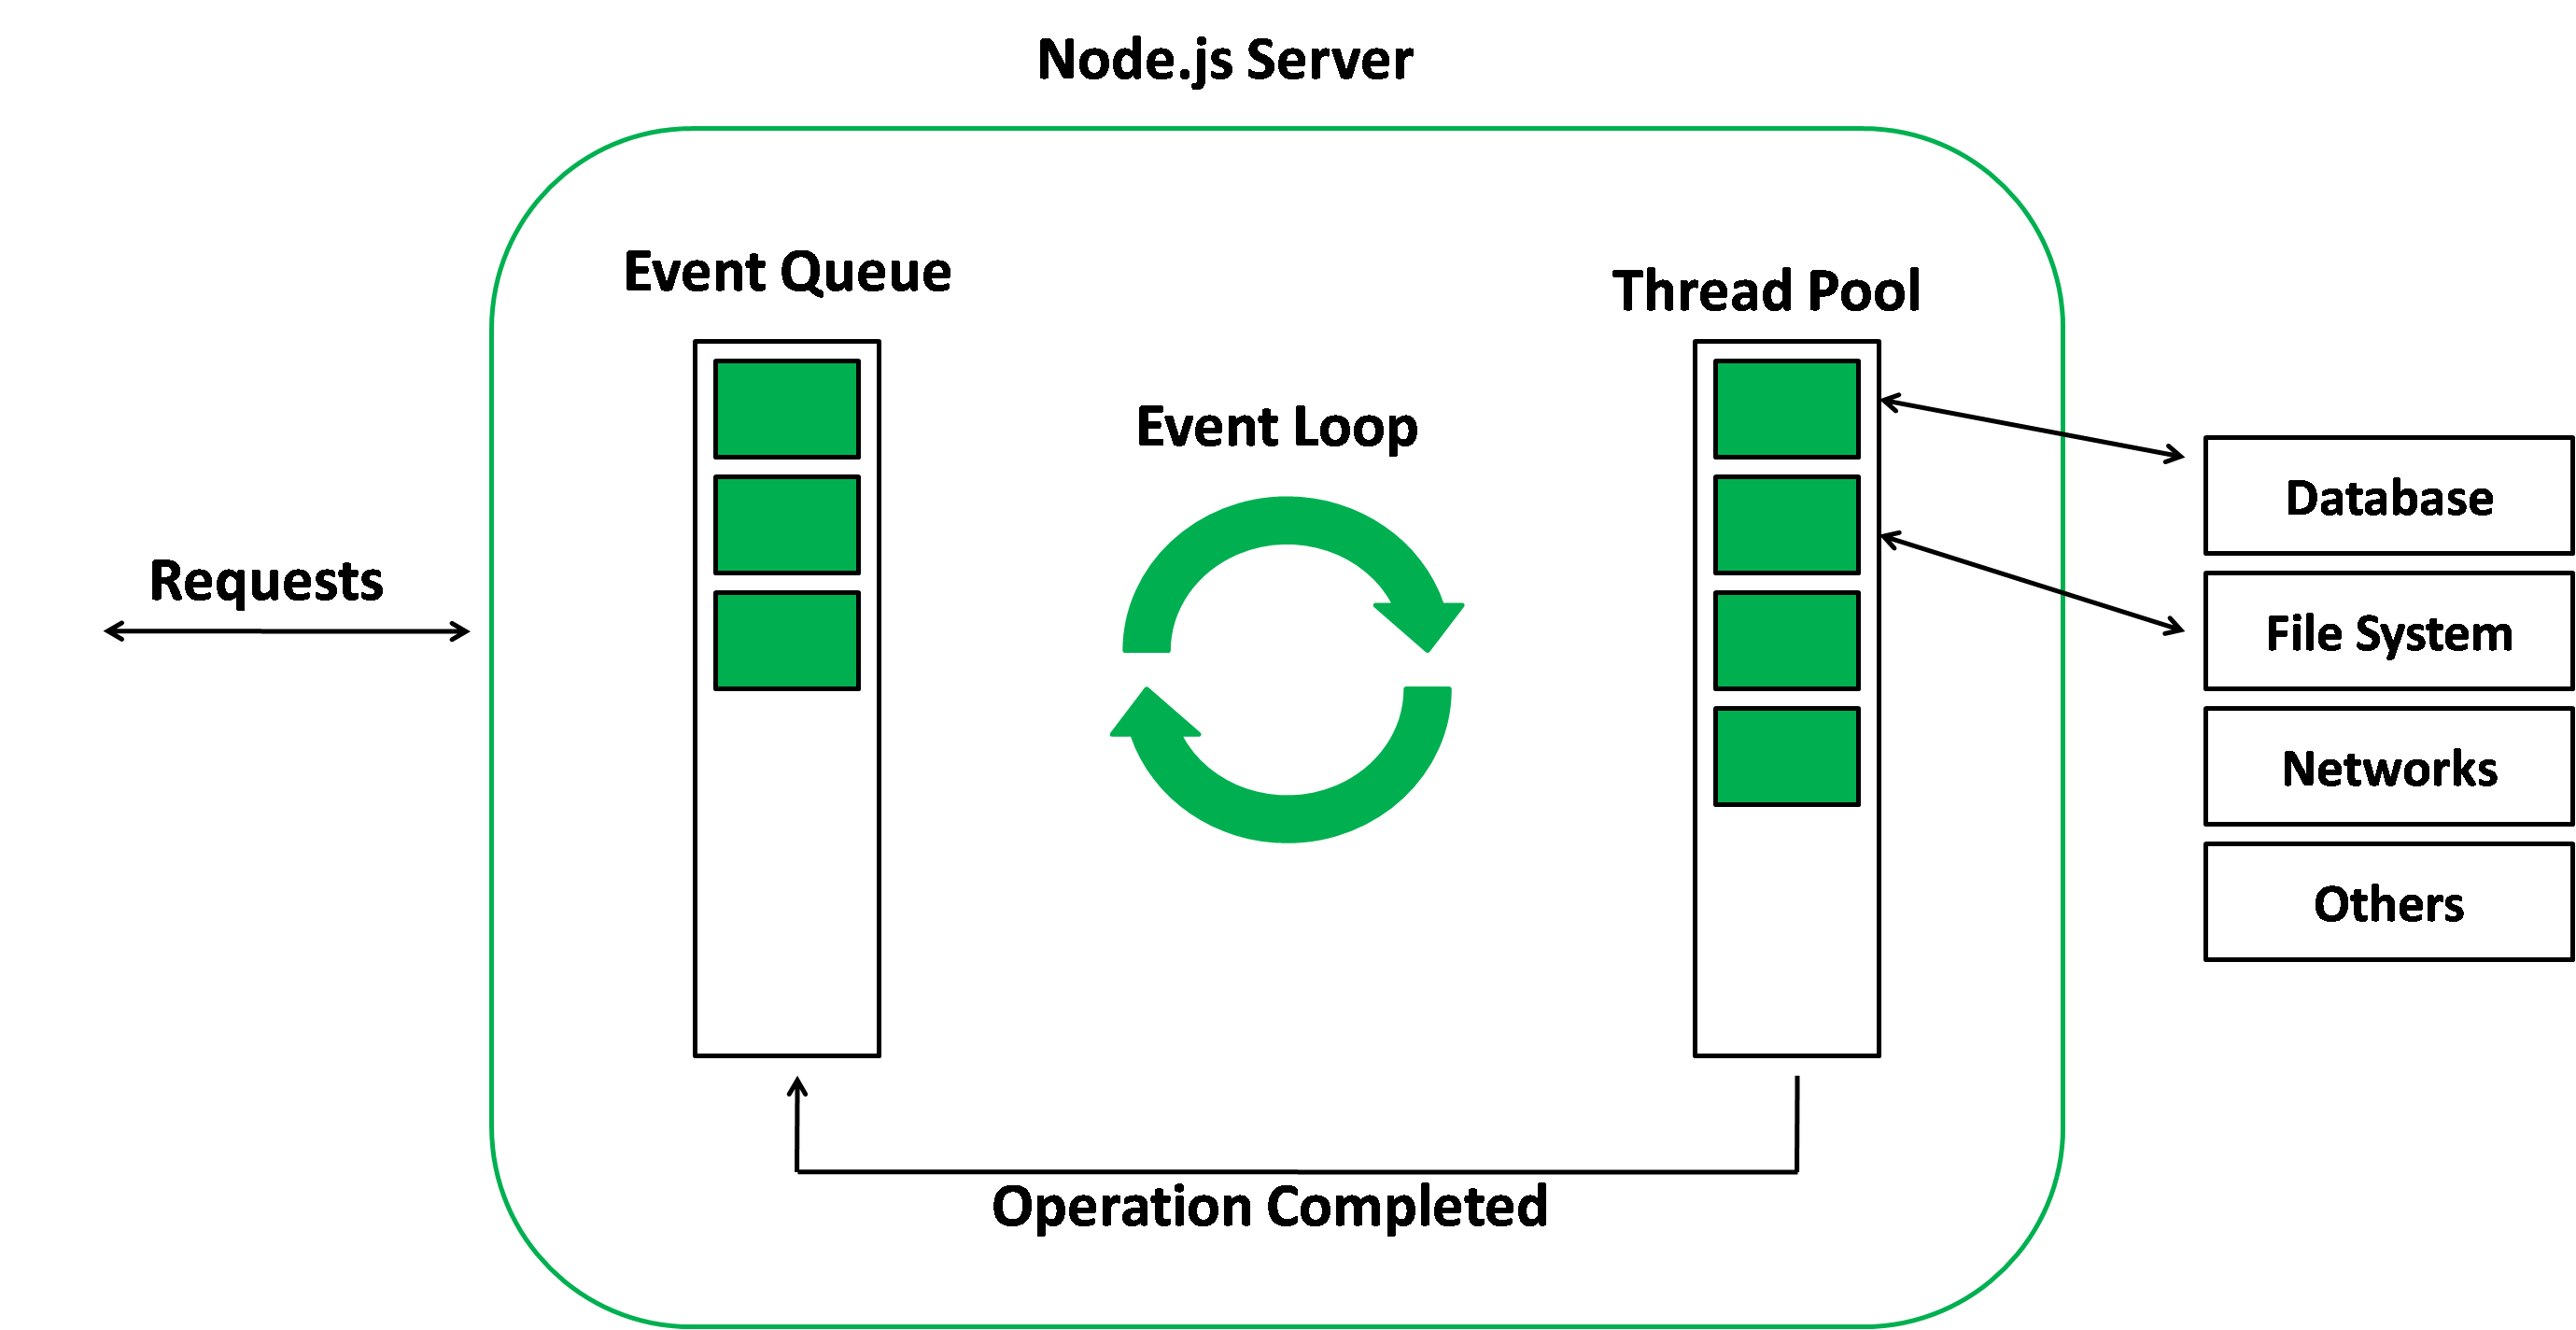
\includegraphics[width=8cm]{Images/eventloop.png}
\centering
\caption{The Node.JS Event Loop}
\label{fig:eventloop}
\end{figure}



The blockchain is actually stored in a LevelDB database. LevelDB is a simple embedded key-value storage engine that provides an ordered mapping from string keys to string values. Moreover, it provides basic operations, for example:
\begin{itemize}
\item[\adforn{43}] \texttt{put(key,value)} that insert value with the given key inside the DB (if the value is already defined, it will override its value with the new one)
\item[\adforn{43}] \texttt{get(key)} that given a key, it will return the associated value (or null if the value is not in the DB)
\item[\adforn{43}] \texttt{delete(key)} that removes the given key (if present) from  the DB.
\end{itemize}

The blockchain data is replicated in every node of the system. When a new node is started, it will reach out to a known node to be registered in the network. Every node keeps the list of registered peers and they exchange their peers list to keep track of new or lost peers.

Once a node has entered the network it starts a procedure called \textit{Initial Block Download}: it asks for the longest chain and it downloads the missing blocks from a random peer.

Once it has downloaded the whole blockchain, the node is said to be active and it can perform queries or add new transactions. Every node tries to mine a new block in an asynchronous way. When a node mines a block it announces it to all the others nodes in the system.

Each node consists of two services: front-end and back-end. The front-end is a static React web app that handles the user input and communicate with an API to the back-end in order to fetch the data it needs. In our particular case, when a user wants to add a flight into the system, it can access the front-end interface, which provides a form, and insert the data. Once the form is correctly filled, the flight is inserted in a queue and it waits until a node in the network mines a block containing all the transactions that are currently contained in the queue. Using the front-end application a user can also make queries to fetch routes and flights. These operations (insertion and searching) can also be performed by calling directly the back-end, using the pre-defined POST and GET endpoints, passing the information in a JSON format.

\section{Second Task}

After we implemented our application we wanted to analyse its performance and scalability properties. In order to do so, we used \textit{Tsung}\footnote{Tsung is an high-performance benchmark framework.} to perform some benchmarks.

To perform the benchmarks we used two different machines: the server (described previously) and another identical Linux machine, directly connected via wired network and a Gigabit Ethernet switch. We have done this do avoid performance drops due to the benchmark software.




\paragraph*{1. Imagine the system as a monolithic queue and measure its expected service time and its second moment.} \mbox{}\\\\ 

In order to do so, we setup a customer to make a query, wait for the answer and then leave the system. 
This kind of setup ensures that every request is independent from the previous ones. 
The first step was to run a single test with this setup to decide which query was the slowest, in this way we could use just for our benchmarks since it would represent a good indicator for a heavy load. 
We did this because if we used the fastest query for the benchmark we would produce a biased result. We found that the heaviest query is the one that states: \textit{"given a pair of cities A and B, and a time interval, count the number of flights connecting city A to city B"}.\\

% TODO — TABELLINA RESPONSE TIME MEDIO DELLE VARIE QUERY 

The second step we did was to run 30 separate tests like the one before, choosing randomly the parameters of the query (To avoid biased results like before) and we were able to obtain the expected service time and its variance. Which resulted to be, respectively 2330.0 ms and 5389.028 ms.
Notice that we were able to retrieve the expected service time from the response time, since having just one customer at the time in a system is in practice the same as setting to zero the waiting time, consequently the response time must correspond only to the service time. 

\paragraph*{2. Perform the test as open system with different workload intensities: 0.3L, 0.5L, 0.8L, 0.85L, where L is the maximum arrival rate determined from the expected service time estimated at point 1. Compare the measures with the lines predicted by the M/G/1 and M/G/1/PS queueing systems and discuss the results.} \mbox{}\\\\

The maximum arrival rate is given by the maximum throughput of the bottleneck (In this particular case we are considering to have just 1 station, so we know which one is the bottleneck) and the maximum throughput at the bottleneck is given by its service rate.

At this point we want to compute the theoretical values of expected response time and expected number of jobs supposing we have an M/G/1 and an M/G/1/PS queue, so that then we can compare these measures with the ones obtained from the benchmarks.

We know in general that response time is given by the expected waiting time plus the service time, in particular: 
\begin{itemize}
\item[\adforn{43}] In the M/G/1 setting the expected waiting time is given by $$E[W]=\dfrac{\rho+\lambda\mu\sigma^2}{2(\mu-\lambda)}$$ and assuming stability the expected service time is given by $\dfrac{1}{\mu}$, therefore:
$$\bar{R}=E[W]+\dfrac{1}{\mu} .$$

This means that in this setting the expected number of jobs is given by the expected number of jobs in the waiting room plus the ratio of users being served, i.e.
\begin{align*}
E[N_W] &= \lambda E[W]\\
E[N] &= E[N_W]+\dfrac{\lambda}{\mu}
\end{align*}

\item[\adforn{43}] In the M/G/1/PS setting we know expected response time and number of jobs do not depend on the variance and correspond to the measures we use for M/M/1 systems; i.e.:

\begin{align*}
\bar{R} &= \dfrac{1}{\mu-\lambda}\\
\bar{N} &= \dfrac{\rho}{1-\rho}
\end{align*}
\end{itemize}

Using this we found the following theoretical data (RespTime and NumJobs stand for the expected response time and the expected number of jobs, respectively):

\begin{table}[H]
\centering
\begin{tabular}{c|c|c|cc}
\multicolumn{1}{l|}{}         & \multicolumn{2}{c|}{M/G/1}                                                        & \multicolumn{2}{c}{M/G/1/PS}                                                     \\ \hline
\multicolumn{1}{l|}{Workload} & \multicolumn{1}{l|}{RespTime (ms)} & \multicolumn{1}{l|}{NumJobs} & \multicolumn{1}{l|}{RespTime (ms)} & \multicolumn{1}{l}{NumJobs} \\ \hline
0.3                           & 2829.78                            & 0.36                                         & \multicolumn{1}{c|}{3328.57}       & 0.43                                        \\
0.5                           & 3496.16                            & 0.75                                         & \multicolumn{1}{c|}{4660.0}        & 1.0                                         \\
0.8                           & 6994.63                            & 2.40                                         & \multicolumn{1}{c|}{11650.0}       & 4.0                                         \\
0.85                          & 8938.22                            & 3.26                                         & \multicolumn{1}{c|}{15533.33}      & 5.67                                       
\end{tabular}
\end{table}

Below this, we show the table containing the data found with the benchmark of our application:

\begin{table}[H]
\centering
\begin{tabular}{c|c|c|}
\multicolumn{1}{l|}{Workload} & \multicolumn{1}{l|}{RespTime (ms)} & \multicolumn{1}{l|}{NumJobs} \\ \hline
0.3                           & 3036.72                            & 0.39                         \\
0.5                           & 3716.63                            & 0.83                         \\
0.8                           & 6981.09                            & 2.13                         \\
0.85                          & 9562.70                            & 3.62                        
\end{tabular}
\end{table}

Comparing the two tables we can notice that our empirical measurements are closer to the M/G/1 theoretical values. 

% TODO — MORE CONSIDERATIONS!

\paragraph*{3. Propose a queueing network model of your application where you distinguish at least three stations: disk, processor and a station modeling the thinking time of the requests. Parametrize the queueing network based on the measurements you can do on your application.} \mbox{}\\\\

We modelled our queuing network based on considerations from our implementation:

\begin{itemize}
\item[\adforn{43}] Once a request is received, a disk read is immediately enqueued to fetch the blocks from the database;
\item[\adforn{43}] All the blocks are fetched from the LevelDB database, reading from the disk;
\item[\adforn{43}] Once all blocks are read, they are filtered and processed using a blocking CPU process.
\end{itemize}

Therefore, the system can be modelled as a three-stations closed-loop queuing network (figure \ref{fig:img1}).

\begin{figure}[h]
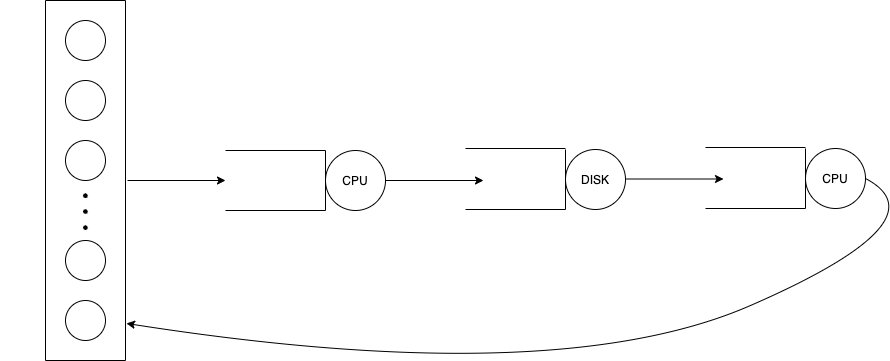
\includegraphics[width=10cm]{Images/img1.png}
\centering
\caption{Model with three stations}
\label{fig:img1}
\end{figure}

This approach, however, it's problematic due to the nature of Node.JS, since it becomes difficult to benchmark the utilization of the two CPUs stations. For this reason we choose a simpler model (figure \ref{fig:img2}), with a single CPU station, since the time required to read the request and start the disk read is much lower than the time required to perform the filtering and aggregation.

\begin{figure}[h]
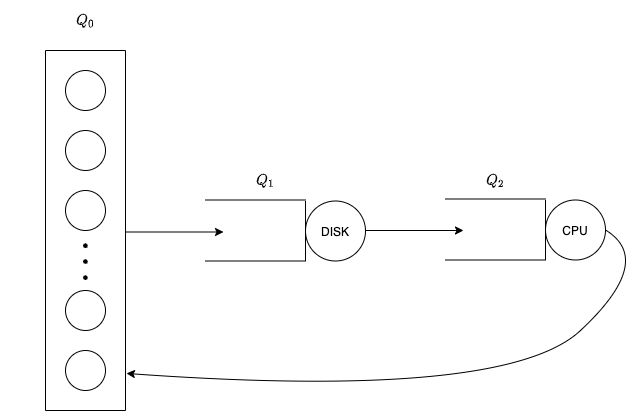
\includegraphics[width=10cm]{Images/img2.png}
\centering
\caption{Model with two stations}
\label{fig:img2}
\end{figure}

As \textbf{thinking time} we have choosen a resonable value of $10$ seconds: once an user receieves the results from the server, we expect him to spend some time to read them before making another request.

To perform further analysis on this model, we needed to find the service times of the two station. To do so we performed another closed-loop benchmark with Tsung, using a single user and no thinking time. While performing the benchmark we used the \textbf{iostat} tool to monitor the usage of the disk and the CPU. Using the command \texttt{iostat -x sda 30} we sampled the utilization of our disk every 30 seconds. To find the utilization of the CPU we used the \texttt{\%user} field. After reading 30 samples (10 minutes of data), we calculated an average of the two 




\end{document}
